\documentclass[11pt]{article}

\usepackage[utf8]{inputenc}
\usepackage[T1]{fontenc}
\usepackage[margin=1in]{geometry}
\usepackage{amsmath}
\usepackage{booktabs}
\usepackage{xcolor}
\usepackage{caption}
\usepackage{listings}
\usepackage{tikz}
\usetikzlibrary{arrows.meta,positioning,calc}
\usepackage[hidelinks]{hyperref}

% ── Listing style ───────────────────────────────────────────────────────
\definecolor{codebg}{rgb}{0.96,0.96,0.97}
\definecolor{codekw}{rgb}{0.10,0.30,0.65}
\lstset{
  basicstyle=\ttfamily\small,
  backgroundcolor=\color{codebg},
  frame=single,
  framesep=4pt,
  breaklines=true,
  columns=fullflexible,
  keepspaces=true,
  showstringspaces=false
}

% ── TikZ shared styles ──────────────────────────────────────────────────
\tikzset{
  box/.style={draw, rounded corners=2pt, minimum height=9mm, minimum width=20mm,
              align=center, font=\small, fill=white},
  cloud/.style={box, fill=blue!6},
  local/.style={box, fill=green!8},
  edge/.style={-{Stealth[length=2mm]}, thick},
  dedge/.style={-{Stealth[length=2mm]}, thick, dashed}
}

\title{\textbf{BridgeHook: A Zero-Install Webhook Bridge\\Using a Browser Extension as the Forwarding Agent}}

\author{Halleluyah Oludele\\
College of Medicine, University of Ibadan, Ibadan, Nigeria\\
\texttt{halleluyaholudeele@gmail.com}}

\date{June 2026}

\begin{document}
\maketitle

\begin{abstract}
Testing webhooks against a service running on localhost normally requires a public ingress: developers install a reverse-tunnel daemon (ngrok, cloudflared, localtunnel) or run a relay client (smee-client, gosmee) that subscribes to a hosted endpoint and re-POSTs payloads locally. Both add an install step and a long-lived local process. BridgeHook removes the install: the forwarding agent is a browser extension the developer already has a browser to run. The relay+SSE-to-localhost pattern itself is not new --- smee.io, gosmee, and similar tools predate this work and are credited throughout. BridgeHook's contribution is a composition: a zero-install webhook bridge that uses a browser extension as the forwarding agent (escaping the CORS / Private-Network-Access wall that blocks page-JavaScript relays), backed by a Cloudflare Durable Object rendezvous, with per-event cryptographic request signing (an untrusted-relay model) and a hybrid push/poll delivery scheme resilient to the Manifest V3 service-worker lifecycle. We describe the architecture, trace every mechanism to the shipping implementation, give a qualitative feature comparison against existing tools, and specify a reproducible latency methodology. The tool runs today on Cloudflare Workers free-tier hosts; a custom-domain deployment is designed but not yet provisioned. We state the limitations plainly: Chromium/MV3 only, single-region relay, and dependence on the relay operator (mitigated, not eliminated, by signing).
\end{abstract}

\section{Introduction}
\label{sec:intro}

A webhook is an HTTP request a third-party service (Stripe, GitHub, a payment
processor) sends to a developer-configured public URL when an event
occurs~\cite{stripewebhooks,githubwebhooks}. During development the handler
under test runs on \texttt{localhost}, which has no public address. The
standard remedy is to publish localhost to the internet, then point the webhook
source at the published URL.

Two families of tools do this. \emph{Reverse tunnels} (ngrok, cloudflared,
localtunnel, Pinggy) run a local agent that opens an outbound connection to a
cloud endpoint and exposes a public hostname bound to a local
port~\cite{ngrok,cloudflaretunnel,localtunnel,pinggy}. \emph{Relay clients}
(smee-client, gosmee) subscribe over Server-Sent Events (SSE)~\cite{htmlsse} to
a hosted channel and re-issue each received payload as a local HTTP
request~\cite{smeeclient,gosmee}. Each approach asks the developer to install
something --- a binary, an npm package, an SSH invocation --- and to keep a
local process alive for the duration of the session.

This paper describes BridgeHook, which keeps the relay+SSE design but moves the
forwarding agent into a browser extension. A developer who has a Chromium
browser open --- which a web developer does --- adds the extension once and
needs no per-project install, no daemon, and no terminal. The thesis is narrow:
the install friction of local webhook testing is removable by reusing the
browser as the always-present forwarding host, provided the agent runs as an
extension rather than as page JavaScript. Section~\ref{sec:background} explains
why page JavaScript cannot do this and an extension can.

This paper makes the following contributions:
\begin{enumerate}
  \item \textbf{Extension-as-agent forwarding.} We identify the browser
        extension as the one client form that can legally forward an
        HTTPS-relayed webhook to an \texttt{http://localhost} target, and show
        why a page-JavaScript relay (an approach that already
        exists~\cite{hookslocalhost}) cannot
        (Section~\ref{sec:background}).
  \item \textbf{A Durable Object rendezvous and a hybrid push/poll delivery
        scheme} resilient to the Manifest V3 service-worker lifecycle
        (Sections~\ref{sec:relay},~\ref{sec:hybrid},~\ref{sec:mv3}).
  \item \textbf{An untrusted-relay signing model}: per-event ECDSA signing of
        privileged client calls so a malicious or compromised relay cannot
        forge them, with the guarantee's exact scope and limits stated
        (Section~\ref{sec:security}).
  \item \textbf{A qualitative comparison} against eight existing tools and a
        reproducible latency methodology (Section~\ref{sec:eval}), with the
        implementation released as open source (Artifact Availability).
\end{enumerate}
The relay+SSE transport itself is inherited from prior tools and is not claimed
as novel; the contribution is the composition above.

\section{Background and Browser Constraints}
\label{sec:background}

\paragraph{Webhooks.} A producer POSTs an event body and headers (often an
HMAC signature) to a configured URL and expects a timely HTTP response; the
response status is used for retry decisions~\cite{stripewebhooks,githubwebhooks}.
A local-testing tool must therefore both deliver the request to localhost and
return the local handler's response to the producer.

\paragraph{Reverse tunnels.} ngrok, cloudflared, localtunnel, and Pinggy
establish an outbound connection from a local agent and bind a public hostname
to a local port~\cite{ngrok,cloudflaretunnel,localtunnel,pinggy}. Pinggy reuses
the system SSH client, avoiding a bespoke binary, but still requires a running
SSH session and (on the free tier) reissues the URL after a timeout.

\paragraph{Relay plus SSE.} smee.io exposes a public channel URL; the
smee-client connects to it over SSE and re-POSTs payloads to a local
target~\cite{smeeio,smeeclient}. gosmee reimplements both halves in Go and lets
operators self-host the relay~\cite{gosmee}. svix and Hookdeck provide
production webhook infrastructure with CLIs whose \texttt{listen} subcommand
forwards to localhost~\cite{svixcli,hookdeck}; Webhook Relay offers the same
forward-to-localhost capability through a CLI or container
agent~\cite{webhookrelay}. BridgeHook's relay and SSE transport are this same
pattern. What differs is the client: an extension, not a local process.

\paragraph{The browser security wall.} If the forwarding agent were ordinary
page JavaScript served over HTTPS, three browser policies would block it from
reaching \texttt{http://localhost}:
\begin{itemize}
  \item \textbf{Mixed content:} an HTTPS page may not issue a plain-HTTP
        subresource request, so \texttt{fetch("http://localhost:3000/...")}
        from an HTTPS dashboard is blocked or silently upgraded~\cite{mdnmixedcontent}.
  \item \textbf{CORS:} a cross-origin response without permissive
        \texttt{Access-Control-Allow-*} headers is not readable by page script;
        a local dev server rarely sets these for an arbitrary cloud origin.
  \item \textbf{Private Network Access (PNA):} the WICG draft (formerly
        CORS-RFC1918) restricts requests originating in a public context that
        target a private/local endpoint; Chrome sends a CORS preflight
        (\texttt{Access-Control-Request-Private-Network: true}) the local
        server must explicitly answer~\cite{pna,pnapreflight}.
\end{itemize}
A browser \emph{extension} with an explicit \texttt{host\_permissions} grant
for \texttt{http://localhost/*} is not subject to these page-context
restrictions for its own \texttt{fetch} calls; the user authorizes the local
reach at install time. This is the single capability that lets the extension
forward an HTTPS-relayed request to an HTTP localhost target, and it is why the
agent must be an extension rather than a tab. A tab-based relay of exactly this
shape exists: hooks-localhost broadcasts received webhooks over WebSocket to an
open page, which then \texttt{fetch}es localhost~\cite{hookslocalhost}. It works
only when the local dev server returns permissive CORS headers to the relay's
origin, and only while the tab stays open. Moving the agent into an extension
removes both constraints --- the CORS-allowlist dependency and the kept-open
tab. (Section~\ref{sec:limits} returns to the standing risk that PNA-style rules
may eventually constrain extensions too.)

\section{Design}
\label{sec:design}

Figure~\ref{fig:dataflow} shows the end-to-end path. The relay never contacts
localhost; the extension is the only component that does.

\begin{figure}[t]
\centering
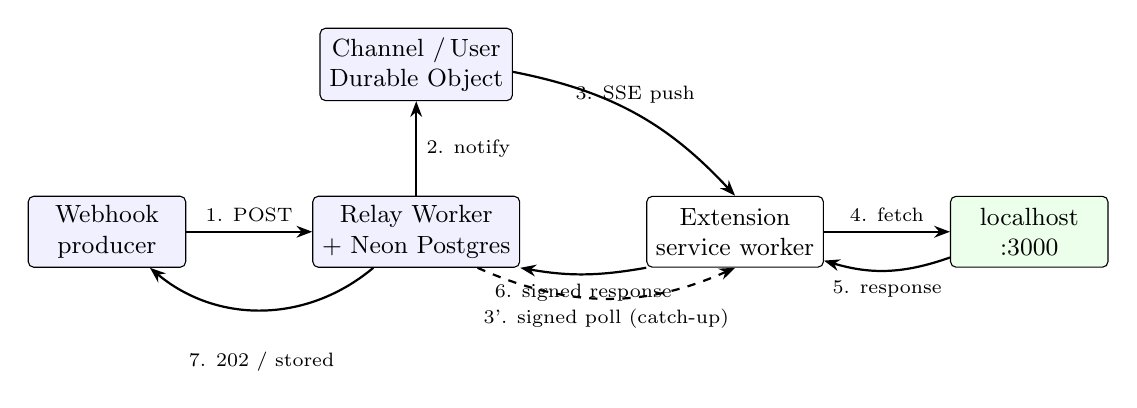
\begin{tikzpicture}[node distance=10mm and 16mm]
  \node[cloud] (prod) {Webhook\\producer};
  \node[cloud, right=of prod] (relay) {Relay Worker\\+ Neon Postgres};
  \node[cloud, above=12mm of relay] (do) {Channel /\,User\\Durable Object};
  \node[box, right=of relay] (ext) {Extension\\service worker};
  \node[local, right=of ext] (local) {localhost\\:3000};

  \draw[edge] (prod) -- node[above,font=\scriptsize]{1. POST} (relay);
  \draw[edge] (relay) -- node[right,font=\scriptsize]{2. notify} (do);
  \draw[edge] (do) to[bend left=18] node[above,font=\scriptsize]{3. SSE push} (ext.north);
  \draw[dedge] (relay) to[bend right=24] node[below,font=\scriptsize]{3'. signed poll (catch-up)} (ext.south);
  \draw[edge] (ext) -- node[above,font=\scriptsize]{4. fetch} (local);
  \draw[edge] (local) to[bend left=18] node[below,font=\scriptsize]{5. response} (ext);
  \draw[edge] (ext.south west) to[bend left=10] node[below,font=\scriptsize]{6. signed response} (relay.south east);
  \draw[edge] (relay) to[bend left=40] node[below=4mm,font=\scriptsize]{7. 202 / stored} (prod);
\end{tikzpicture}
\caption{End-to-end dataflow. The producer's POST is persisted and fanned out
to the extension over SSE (push) with signed polling as catch-up; the extension
forwards to localhost and returns the captured response to the relay, signed.}
\label{fig:dataflow}
\end{figure}

\subsection{Relay: Worker plus Durable Object rendezvous}
\label{sec:relay}

The relay is a Cloudflare Worker built on Hono, backed by Neon
PostgreSQL via Drizzle. Inbound webhooks are accepted either at a path
(\texttt{/hook/:channelId}) or, when a tunnel apex domain is configured, at a
wildcard subdomain (\texttt{<channelId>.<apex>}). Intake validates the channel,
enforces a body-size cap and a path allowlist, applies the per-user daily event
cap, persists an \texttt{events} row, and returns \texttt{202} immediately ---
it never blocks on localhost. Two tables back the system: \texttt{channels}
(id, ECDSA public key, port, allowed paths, owner) and \texttt{events} (request
method/path/headers/body, response status/headers/body, latency, claim
fields).

Live delivery uses Cloudflare Durable Objects~\cite{durableobjects}. A Durable
Object (DO) is a single addressable instance per id, so every SSE connection
and every webhook notification for one channel reach the \emph{same} instance
and can share in-memory state. The \texttt{ChannelDO} holds open SSE writers in
a \texttt{Set}; on intake the Worker POSTs a notify to the DO, which fans the
event out to all writers with \texttt{Promise.allSettled} and evicts any writer
whose write rejects (a disconnected client). A per-channel connection cap
rejects excess subscribers with \texttt{429}. A second DO type
(\texttt{UserDO}) fans every event for any channel a signed-in user owns to a
single cross-channel stream, which is what the extension subscribes to in
push mode.

Authentication on the relay is gated by a single secret: when
\texttt{BETTER\_AUTH\_SECRET} is set the relay runs in hosted mode with
Better-Auth sessions and device tokens; when unset it runs in self-host mode
with an implicit user and no auth routes. To stay within the Workers free-tier
10\,ms CPU budget, password hashing uses a hand-rolled PBKDF2 rather than a
heavier KDF.

\subsection{Extension bridge: the forwarding agent}
\label{sec:bridge}

The extension is Manifest V3 with a module service worker, the permissions
\texttt{storage}, \texttt{notifications}, \texttt{alarms}, and
\texttt{host\_permissions} for \texttt{http://localhost/*} plus the relay hosts.
The localhost grant is the capability discussed in
Section~\ref{sec:background}; with it the service worker's \texttt{fetch} to
\texttt{http://localhost:PORT} is exempt from the page-context CORS and
mixed-content rules that block a tab.

For each event the worker reconstructs the local request, strips
infrastructure headers that must not be replayed (\texttt{host},
\texttt{cf-*}, \texttt{x-forwarded-*}, \texttt{content-length},
\texttt{transfer-encoding}, and similar), issues the \texttt{fetch} to
localhost, measures latency with \texttt{performance.now()}, captures status,
headers, and body, and returns that response to the relay. A connection refusal
is reported to the user as a desktop notification rather than silently dropped.

\subsection{Hybrid push/poll delivery}
\label{sec:hybrid}

Delivery uses two paths feeding one handler. In \emph{push} mode (available
when the user is signed in via the dashboard session cookie) the worker holds a
streaming-fetch SSE connection to \texttt{/api/me/stream}; the relay pushes a
\texttt{webhook} frame the instant the event lands, and forwarding starts within
milliseconds. In \emph{poll} mode a per-service loop calls the signed events
endpoint as catch-up and as the sole path when push is unavailable (self-host,
device-token auth, or a dropped stream). A \texttt{Set} of handled event ids is
shared across both paths, so an event delivered by push is filtered out of the
next poll.

The poll cadence is adaptive: 2\,s by default; 15\,s while the SSE stream is
healthy (polling is then only a safety net); 10\,s after more than three
consecutive errors; and 30\,s when the relay reports the daily quota is
exhausted (\texttt{402} with \texttt{code:"quota"}). The SSE reader reconnects
with exponential backoff capped at 30\,s.

\subsection{MV3 service-worker resilience}
\label{sec:mv3}

A Manifest V3 background service worker is event-driven and is terminated on
inactivity; any in-flight \texttt{setTimeout} loop dies with
it~\cite{mv3swlifecycle}. A naive polling loop would therefore stop whenever
Chrome reclaims the worker. BridgeHook treats the worker as disposable and
rebuilds state on each wake (Figure~\ref{fig:mv3}). A \texttt{chrome.alarms}
heartbeat fires every 30\,s --- the MV3 minimum period --- and, on
\texttt{onInstalled}, \texttt{onStartup}, and every cold boot, the worker
\emph{rehydrates}: it reloads services from \texttt{chrome.storage}, refreshes
account state, and re-attaches a polling loop for any active service whose
in-tick loop died. The user SSE stream is restarted if it died with the worker.
Signing keys live in IndexedDB and survive worker death; a service whose key is
missing is skipped rather than run unsigned.

\begin{figure}[t]
\centering
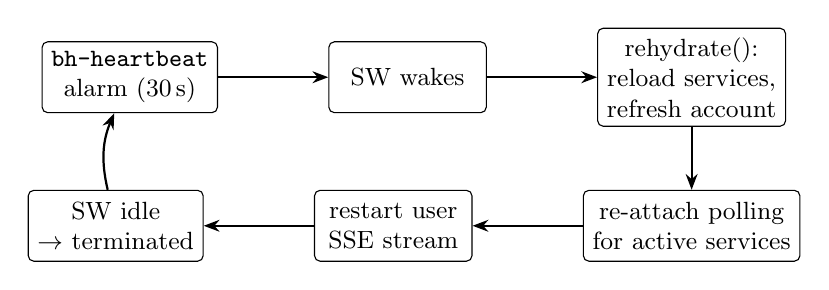
\begin{tikzpicture}[node distance=8mm and 14mm]
  \node[box] (alarm) {\texttt{bh-heartbeat}\\alarm (30\,s)};
  \node[box, right=of alarm] (wake) {SW wakes};
  \node[box, right=of wake] (rehy) {rehydrate():\\reload services,\\refresh account};
  \node[box, below=of rehy] (poll) {re-attach polling\\for active services};
  \node[box, left=of poll] (sse) {restart user\\SSE stream};
  \node[box, left=of sse] (idle) {SW idle\\$\rightarrow$ terminated};

  \draw[edge] (alarm) -- (wake);
  \draw[edge] (wake) -- (rehy);
  \draw[edge] (rehy) -- (poll);
  \draw[edge] (poll) -- (sse);
  \draw[edge] (sse) -- (idle);
  \draw[edge] (idle) to[bend left=18] (alarm);
\end{tikzpicture}
\caption{MV3 resilience loop. The worker is assumed to die between alarm ticks;
each wake rebuilds the polling loops and SSE stream from durable storage rather
than relying on in-memory continuity.}
\label{fig:mv3}
\end{figure}

\subsection{Security model}
\label{sec:security}

The relay is treated as untrusted for integrity. Each channel owns a
\emph{non-extractable} ECDSA P-256 keypair generated in the browser via Web
Crypto and stored in IndexedDB; only the raw public key is sent to the relay at
channel creation. Every privileged client call (fetch events, post response,
claim) is signed: the client builds a canonical string over method, path,
timestamp, and a SHA-256 of the body, signs it, and attaches
\texttt{X-BH-Timestamp} and \texttt{X-BH-Signature}
(Listing~\ref{lst:canonical}). The relay re-derives the same string and
verifies against the stored public key within a 60\,s clock-skew window.
Because the private key never leaves the browser and is non-extractable, a
relay operator (or anyone who hijacks the SSE stream) can observe and reorder
frames but cannot \emph{forge} a signed claim or response. The scheme provides
integrity and authenticity, not full anti-replay: the canonical string carries
a timestamp but no nonce, and the relay keeps no used-signature cache, so a
captured signed request can be replayed within the 60\,s window. This is benign
for the operations that are signed --- the response upload is idempotent and the
claim is a single-winner atomic update (control 3 below) --- but it is not a
general replay guarantee. The signature covers the path but not the query
string, so query parameters (such as a result \texttt{limit}) are
unauthenticated; no privileged decision depends on them.

\begin{lstlisting}[caption={Canonical string signed per request (client and relay derive it identically).},label={lst:canonical},language=,float=t]
canonical = METHOD + "\n"
          + pathname + "\n"
          + timestamp + "\n"
          + sha256_hex(body)
// headers: X-BH-Timestamp, X-BH-Signature (ECDSA P-256 / SHA-256)
\end{lstlisting}

Three further controls round out the model. (1) A per-channel \emph{path
allowlist} is enforced server-side at intake: a webhook whose post-prefix path
is not in the channel's allowed set is rejected with \texttt{403}, so a leaked
channel id cannot be used to drive arbitrary local routes (an empty allowlist
permits any path, but the extension always sets a non-empty list at channel
creation). (2) Authentication
is three-tier in priority order: a dashboard session cookie
(\texttt{SameSite=None}, sent with \texttt{credentials: "include"}, requiring no
pairing); a long-lived device-token bearer (\texttt{dvc\_...}) minted through an
OAuth-style device-pairing flow for headless or signed-out use; and anonymous,
permitted only against self-host relays. (3) Multiple executors on one channel
(extension, dashboard tab, desktop app) arbitrate via an atomic claim ---
\texttt{UPDATE \ldots\ WHERE claimed\_by\_device\_id IS NULL} --- so exactly one
forwards each event.

\subsection{Stable URLs and port detection}
\label{sec:stable}

A webhook URL pasted into Stripe must remain valid across browser restarts and
worker deaths. When a signed-in user re-adds a service for a port that already
has a channel, the extension reuses the existing channel id rather than minting
a new one. If the local private key is gone (cleared storage, fresh profile),
the extension generates a new keypair and re-keys the existing channel via a
rotate-key call, keeping the same id and URL with fresh signing material. To
reduce setup friction, the extension can HEAD-probe a set of common development
ports (3000, 3001, 4000, 5000, 5173, 8000, 8080, 8888) and suggest the live
ones.

\section{Implementation}
\label{sec:impl}

BridgeHook is a pnpm monorepo. \texttt{packages/shared} holds TypeScript types,
constants, and the Drizzle schema; \texttt{relay/} is the Cloudflare Worker
(Hono + Neon + Better-Auth); \texttt{apps/web} is the Vite/React landing page
and dashboard; \texttt{apps/extension} is the MV3 extension; and
\texttt{apps/desktop} is a planned Tauri tray app that would run the same bridge
loop in Rust for users who want forwarding without a browser open. The DO-based
relay and the ECDSA-signed client protocol are shared by the web dashboard, the
extension, and (by design) the desktop bridge.

\paragraph{Deployment topology.} The intended layout maps three properties to
three subdomains of an apex (\texttt{bridgehook.dev} for docs,
\texttt{app.bridgehook.dev} for the dashboard, \texttt{relay.bridgehook.dev}
for the Worker). \textbf{That apex is not yet registered.} The tool currently
runs on Cloudflare-provided hosts (\texttt{*.workers.dev} for the relay,
\texttt{*.pages.dev} for the web app); the custom-domain layout is the
deployment design, not a live claim. Everything fits Cloudflare's free tier
(Table~\ref{tab:cost}); the relay is stateless per request and DOs hold channel
state in memory, so there is no separate database cost beyond Neon's free tier
for durable event history.

\begin{table}[t]
\centering
\caption{Cloudflare free-tier allowances used by the relay deployment (from the
project's deployment notes). Figures are platform allowances, not measured
load.}
\label{tab:cost}
\begin{tabular}{lll}
\toprule
Service & Free-tier allowance & Hosts \\
\midrule
Cloudflare Pages   & unlimited sites/bandwidth, 500 builds/mo & landing + dashboard \\
Cloudflare Workers & 100{,}000 requests/day, 10\,ms CPU/req   & relay server \\
Durable Objects    & 1M requests/mo, 1\,GB storage            & per-channel + per-user state \\
Custom domain      & $\sim$\$12/year (not yet provisioned)    & \texttt{*.bridgehook.dev} (design) \\
\bottomrule
\end{tabular}
\end{table}

\section{Evaluation}
\label{sec:eval}

\subsection{Feature comparison}
The qualitative comparison in Table~\ref{tab:features} is factual and reflects
each tool's documented behavior~\cite{ngrok,cloudflaretunnel,localtunnel,pinggy,smeeclient,gosmee,svixcli,hookdeck}.
The column where BridgeHook is alone is \emph{install required}: every other
tool ships a binary, an npm package, or an SSH session that must run locally,
whereas BridgeHook's forwarding agent is a browser extension and runs no
separate local process. Per-event request signing toward the relay is the
second distinguishing column.

\begin{table}[t]
\centering
\caption{Qualitative comparison of local webhook delivery tools. ``Local
process'' = a daemon/CLI/SSH session the developer must keep running;
``signing'' = per-event cryptographic signing of the client$\rightarrow$relay
calls; ``delivery'' is the transport model: a held TCP \emph{tunnel},
server-pushed \emph{SSE}, or a \emph{hybrid} of SSE push with polling fallback.}
\label{tab:features}
\small
\begin{tabular}{lccccccc}
\toprule
Tool & No install & No local proc. & No account & Self-host & Per-event sign & Delivery & Free \\
\midrule
ngrok            & no  & no  & no  & no  & n/a & tunnel & freemium \\
cloudflared      & no  & no  & yes & no  & n/a & tunnel & yes \\
localtunnel      & no  & no  & yes & yes & n/a & tunnel & yes \\
Pinggy           & yes\textsuperscript{*} & no & yes & no & n/a & tunnel & freemium \\
smee-client      & no  & no  & yes & yes & no  & SSE & yes \\
gosmee           & no  & no  & yes & yes & no  & SSE & yes \\
svix-cli         & no  & no  & yes & yes & no  & SSE & freemium \\
Hookdeck CLI     & no  & no  & no  & no  & no  & SSE & freemium \\
\textbf{BridgeHook} & \textbf{yes} & \textbf{yes} & yes\textsuperscript{\dag} & yes & \textbf{yes} & hybrid & yes \\
\bottomrule
\end{tabular}
\par\smallskip
\footnotesize\textsuperscript{*}Pinggy needs no binary but requires a running
SSH session. \textsuperscript{\dag}Anonymous use is supported only against a
self-hosted relay; the hosted relay requires an account.
\end{table}

\subsection{Latency methodology}
\label{sec:latency}

We have not yet run the latency benchmark; this subsection specifies the
reproducible methodology and the result tables are left with explicit
placeholders to be filled from real runs. \textbf{No latency or throughput
number in this paper is measured; all are marked ``---''.}

\paragraph{Setup.} A local echo server records server-receive time; a load
generator POSTs $N$ events to the channel URL with a monotonic id and a send
timestamp. We instrument four segments: (S1) producer$\rightarrow$relay intake
(relay receive minus send); (S2) relay$\rightarrow$extension delivery, measured
separately for push (SSE) and poll modes; (S3)
extension$\rightarrow$localhost$\rightarrow$extension (the
\texttt{performance.now()} delta the worker already records as
\texttt{latencyMs}, rounded to whole milliseconds, which bounds S3 reporting
resolution); and (S4) end-to-end (local receive minus producer send).
Each configuration is run for the same event count, warmed, and repeated across
seeds; we report median and p95 per segment, and the distribution must be
stamped with a hardware/region fingerprint (client OS, browser build, relay
region, Neon region, git commit). Push and poll are compared at equal event
load to isolate the SSE latency benefit. A cold-start variant deliberately
idles the MV3 worker until termination, then sends one event, to measure the
alarm-driven wake-and-rehydrate penalty. smee-client and ngrok are run on the
same harness at equal event load as external baselines, so BridgeHook's numbers
are not reported in isolation. Significance between configurations is assessed
with bootstrap confidence intervals on the median rather than parametric tests,
which the seed counts do not justify.

\begin{table}[t]
\centering
\caption{End-to-end latency (ms) --- methodology in \S\ref{sec:latency}. All
cells to be filled from real runs.}
\label{tab:latency}
\begin{tabular}{lcccc}
\toprule
Configuration & S1 intake & S2 delivery & S3 local round-trip & S4 end-to-end \\
     & med / p95 & med / p95 & med / p95 & med / p95 \\
\midrule
BridgeHook push (SSE)       & --- / --- & --- / --- & --- / --- & --- / --- \\
BridgeHook poll (2\,s)      & --- / --- & --- / --- & --- / --- & --- / --- \\
BridgeHook poll (15\,s SSE-healthy) & --- / --- & --- / --- & --- / --- & --- / --- \\
BridgeHook cold MV3 wake    & --- / --- & --- / --- & --- / --- & --- / --- \\
\midrule
smee-client (baseline)      & --- / --- & --- / --- & --- / --- & --- / --- \\
ngrok (baseline)            & --- / --- & --- / --- & --- / --- & --- / --- \\
\bottomrule
\end{tabular}
\end{table}

\subsection{Threats to validity}
\label{sec:threats}
The latency table is unpopulated, so this paper makes no empirical performance
claim; the methodology is specified but its results are future work. The feature
comparison (Table~\ref{tab:features}) reflects each tool's \emph{documented}
behavior, not behavior we re-measured, and vendor tiers change over time. The
planned measurement uses a single client, region, and relay deployment, so
results, once collected, will not generalize across regions without repetition.
The security analysis reasons about the shipping code path; it is not a formal
proof and has not been independently audited.

\section{Limitations}
\label{sec:limits}

\textbf{Chromium and MV3 only.} The shipping extension targets Chromium
(Manifest V3, module service worker); Firefox is not yet supported. The
zero-install claim is relative to having a Chromium browser.

\textbf{Service-worker and tab lifecycle.} The MV3 worker can be terminated at
any time; the heartbeat is bounded below by the 30\,s alarm minimum, so a
poll-only configuration can lag a webhook by up to one heartbeat plus rehydrate
cost after a cold wake. Push mode masks this while the SSE stream is healthy,
but push requires the dashboard session cookie and so is unavailable to
device-token and self-host configurations.

\textbf{Trust in the relay operator.} The relay sees every payload in
plaintext (as do smee.io and any hosted relay). Signing protects integrity ---
a hijacked or malicious relay cannot forge signed claims or responses --- but
does not provide payload confidentiality against the operator. Self-hosting the
relay is the mitigation for users who cannot accept that exposure.

\textbf{Private Network Access for extensions.} The capability the design rests
on --- an extension reaching localhost --- could be narrowed if PNA-style rules
are extended to extension contexts~\cite{pna,pnapreflight}. This is a roadmap
risk we do not control; the desktop (Tauri) bridge is the planned fallback if
the browser path is foreclosed.

\textbf{Single-region relay and free-tier caps.} The relay is a single logical
deployment; cross-region producers pay the intake hop to that region. The
hosted free tier enforces a daily event cap (surfaced as \texttt{402}
\texttt{quota}) and the Workers 10\,ms CPU limit shaped the choice of PBKDF2
over a heavier KDF.

\textbf{Custom domain not provisioned.} \texttt{bridgehook.dev} is not yet
registered; the tool runs on \texttt{*.workers.dev} / \texttt{*.pages.dev}.

\section{Related Work}
\label{sec:related}

Reverse tunnels~\cite{ngrok,cloudflaretunnel,localtunnel,pinggy} publish a local
port directly and are general-purpose (any TCP/HTTP service), but require a
local agent. Relay-plus-SSE tools~\cite{smeeio,smeeclient,gosmee} are the direct
antecedents of BridgeHook's transport; gosmee additionally lets operators
self-host the relay, which BridgeHook also supports. Production webhook
platforms~\cite{svixcli,hookdeck} add durable delivery, retries, and permanent
URLs, with CLIs that forward to localhost for development; Hookdeck in
particular offers permanent free URLs and preserved history, overlapping
BridgeHook's stable-URL goal. The closest antecedent is
hooks-localhost~\cite{hookslocalhost}, which also makes the browser the
forwarding agent, but does so from a page over WebSocket and so inherits the
CORS-allowlist and open-tab constraints of \S\ref{sec:background}; running the
agent as an extension is what removes them. Across these tools the forwarding
agent is either a local process or a CORS-constrained tab. BridgeHook's distinct
position is no-local-process forwarding via an extension agent, combined with
the Durable Object rendezvous and untrusted-relay signing described above.

\section{Conclusion}
\label{sec:conclusion}

BridgeHook removes the install and the local daemon from webhook local-testing
by using a browser extension as the forwarding agent, which is the one client
form that can legally reach \texttt{http://localhost} from an HTTPS-relayed
flow. The relay+SSE transport is inherited from smee.io and gosmee and credited
as such; the engineering contribution is the surrounding system enumerated in
\S\ref{sec:intro}, and in particular the choice to run the forwarding agent as
an extension so it clears the browser's localhost-reach restrictions without a
local process. The system runs today on Cloudflare free-tier hosts. The
remaining work is empirical: the latency methodology of \S\ref{sec:latency} must
be run to populate Table~\ref{tab:latency}, and the desktop bridge and
custom-domain deployment are designed but not yet shipped.

\section*{Artifact availability}
The implementation is open source at
\url{https://github.com/hallelx2/bridgehook} (commit \texttt{83c10d3} at the
time of writing), released under the MIT License. The repository contains the
relay Worker, the Manifest V3 extension, the web dashboard, and the shared
schema. The relay self-hosts on Cloudflare Workers: setting
\texttt{BETTER\_AUTH\_SECRET} enables hosted multi-tenant mode, and leaving it
unset runs a single-user self-host relay with no auth routes. The latency
harness of \S\ref{sec:latency} will be released under \texttt{paper/eval/}
alongside its result files.

\bibliographystyle{abbrv}
\bibliography{references}

\end{document}
